\section{$R_{\textrm{NL}}(x)$ as we change $\rho$}
Hall effect experiments are generally done in Hall-bars. These are samples of material with a shape like the one in figure \ref{fig:hall-bar}, it also means that more often than not in experimental setups we cannot change $x$ without changing the geometry of the sample.
\begin{figure}[h!]
    \centering
    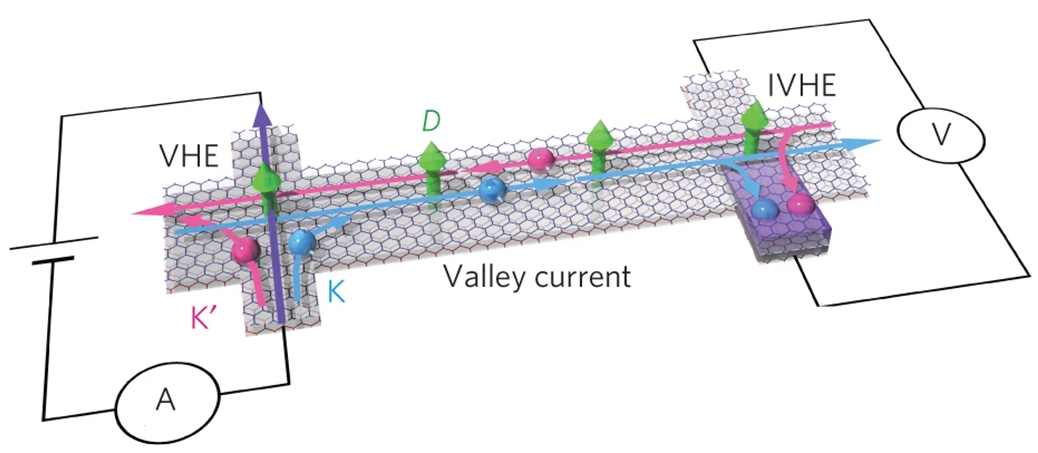
\includegraphics[width=\linewidth]{Immagini/rnl/hallbarbrutta.png}
    \caption{Example of Hall bar the currents are injected and measured in the rectangular contacts that come out from the main strip}
    \label{fig:hall-bar}
\end{figure}\\
In the previous section we studied how $R_{\textrm{NL}}$ depended on $x$, but since Hall-bars can only measure a single $x$ one of the ways to have multiple measurements with the same Hall-bar is to change the resistivity of the material by changing the temperature of the setup, and study $R_{\textrm{NL}}$ as we change $\rho_{xx}$.


If you were to conduct an experiment where you measure $R_{\textrm{NL}}$ as you change the resistivity of the material $\rho$ you would have in general something that looks like figure \ref{fig:rho0}.
\begin{figure}[h!]
    \centering
    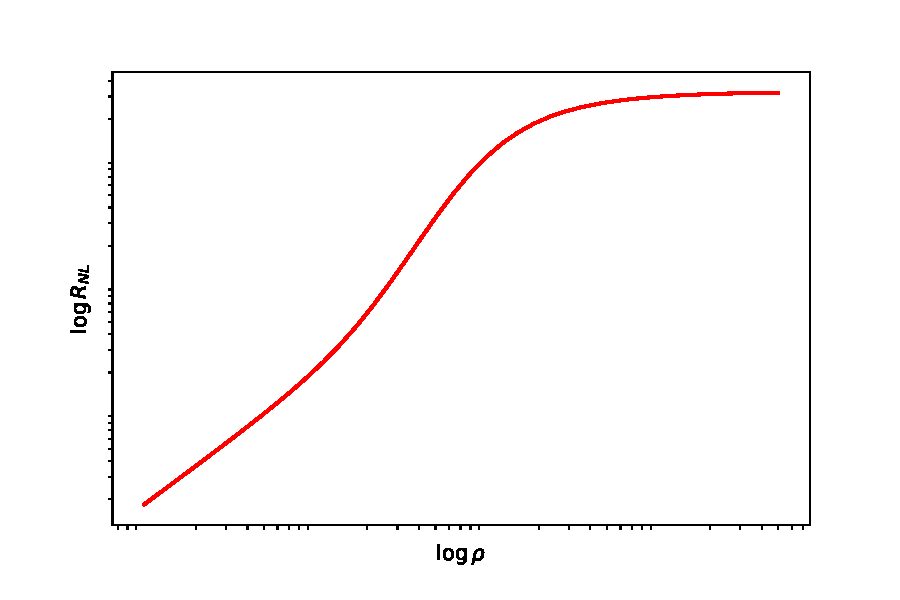
\includegraphics[width=\linewidth]{Immagini/rnl/rho0.pdf}
    \caption{Looking at the image you can see that at the start it increases linearly, then it starts to increase even faster just before reaching a plateau.}
    \label{fig:rho0}
\end{figure}\\
The objective of this section is effectively to be able to understand this graph.

Just like before to understand the general behavior of $R_{\textrm{NL}}(\rho)$ we'll examine $\rho\to 0$ and $\rho \to \infty$. For convenience let's re-write equation \ref{eq:rnlk}
\[
    R_{\textrm{NL}}(k)=\frac{2\omega(k)}{k\sigma_c}
    \bigg\{
        \frac{\omega(k)}{\tanh(kW/2)} + \frac{k\tan^2(\theta_{\textrm{VH}})}{\tanh[\omega(k)W/2]}    
    \bigg\}^{-1}
\]
















\subsection{Low resistivities $\rho\to 0$}
\label{sec:lowrho}
Sending $\rho\to 0$ is effectively equal to sending $\tan(\theta_{\textrm{VH}})=\sigma_{\textrm{v}}\rho\to 0$. To be more precise we are going to assume that
\[
    \frac{k\tan^2(\theta_{\textrm{VH}})}{\tanh[\omega(k)W/2]}\ll \frac{\omega(k)}{\tanh(kW/2)}\quad\quad \forall k  
\]
Which means that $\tan^2(\theta_{\textrm{VH}})\ll 1$. So now we do a Taylor series expansion of the above equation around $\tan^2(\theta_{\textrm{VH}})= 0$.
\[
    R_{\textrm{NL}}(k)\approx R_{\textrm{NL}}(k)|_{\tan^2(\theta_{\textrm{VH}})=0} +
    \frac \partial {\partial \tan^2(\theta_{\textrm{VH}})} R_{\textrm{NL}}(k)|_{\tan^2(\theta_{\textrm{VH}})=0}
\]
that we are going to re-define as
\[
    R_{\textrm{NL}}(k)\approx R_{\textrm{NL}}^{(0)}(k) + R_{\textrm{NL}}^{(1)}(k)\tan^2(\theta_{\textrm{VH}})
\]
The zeroth order term gives us our good old ohmic response in the frequency domain (eq. \ref{eq:ohmick})
\[
    R_{\textrm{NL}}^{(0)}(k)=\frac{2\rho}k\tanh\bigg(\frac{kW}2\bigg)
\]
This makes sense because as we lower $\rho/\rho_{\textrm{v}}$ the hall current will be increasingly smaller and so the ohmic response will dominate.\\
And if we do the Fourier transform to get the $x$ dependent form we get the ohmic nonlocal resistivity \ref{eq:ohmic signal}
\begin{equation}
    R_{\textrm{NL}}^{(0)}(x)=\frac{2\rho}\pi\ln\bigg |\coth \Big(\frac{\pi x}{2W}\Big)\bigg |
\end{equation}
Now let's calculate the first order term

\[
    R_{\textrm{NL}}^{(1)}(k)\tan^2(\theta_{\textrm{VH}})=-2\rho\frac{\omega(k)}k\bigg[\frac{\omega(k)}{\tanh(Wk/2)} \bigg]^{-2}k\frac{\tan^2(\theta_{\textrm{VH}})}{\tanh(\omega(k)W/2)}=
\]
\[
    =-2\rho^3\sigma_{\textrm{v}}^2 \tanh^2\bigg(\frac{kW}2\bigg)\bigg\{\omega(k)\tanh\bigg[\frac{\omega(k) W}2\bigg]\bigg\}^{-1}\equiv
    \rho^3F(k)
\]
where $F(k)$ is defined as follows

\begin{equation}
    F(k)\equiv -2\sigma_{\textrm{v}}^2\tanh^2\bigg(\frac{kW}2\bigg)\bigg\{\omega(k)\tanh\bigg[\frac{\omega(k) W}2\bigg]\bigg\}^{-1}
\end{equation}
And it doesn't depend on $\rho$. Its Fourier transform is 

\begin{equation}
    F(x)=-2\sigma_{v}^2\int_{-\infty}^{+\infty}\tanh^2\bigg(\frac{kW}2\bigg)\bigg\{\tanh\bigg[\frac{\omega(k) W}2\bigg]\bigg\}^{-1}\frac{e^{-ikx}}{\omega(k)}\frac{dk}{2\pi}
\end{equation}
Putting it all together we get that

\begin{equation}
    \lim_{\rho\to 0} R_{\textrm{NL}}(x)=
    \frac{2\rho}\pi\ln\bigg |\coth \Big(\frac{\pi x}{2W}\Big)\bigg | +
    \rho^3F(x) +
    o(\rho^5)
    \label{eq:lowrho}
\end{equation}

PARLARE DEI REGIMI IN CUI DOMINA $\rho^3$



















\subsection{Big resistivities $\rho\to \infty$}
\label{sec:highrho}
Now let's study what happens when $\rho,\tan(\theta_{\textrm{VH}})\to \infty$. First off let's rewrite equation \ref{eq:rnlk} and bring the $\omega(k)$ and $k$ inside the curly braces.
\begin{equation}
        R_{\textrm{NL}}(k)=2\rho
    \bigg\{
        \underbrace{\frac{k}{\tanh(kW/2)}}_{\substack{\text{cannot be}\\\text{ignored for } k=0}} + \frac {k^2}{\omega(k)}\frac{\tan^2(\theta_{\textrm{VH}})}{\tanh[\omega(k)W/2]}    
    \bigg\}^{-1}
    \label{eq:rhoinf1}
\end{equation}

This limit is a bit tricky to evaluate. First off even thought the right-most term inside the curly braces dominates everywhere except for $k=0$ this "\emph{small detail}" is crucial. From image \ref{fig:rho1} we can see that the larger $\rho$ gets, the smaller the area around $k=0$ where the first term dominates.
\begin{figure}[h!]
    \centering
    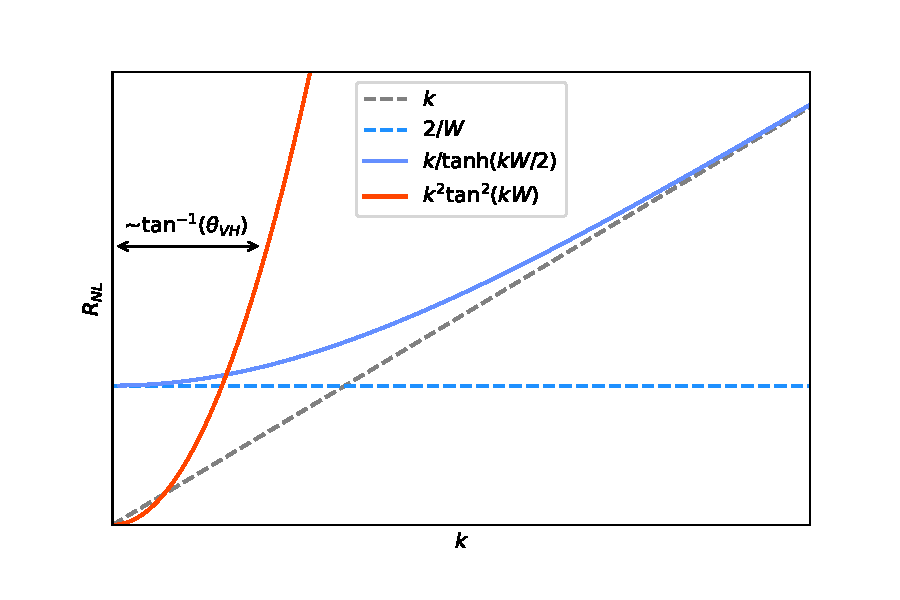
\includegraphics[width=\linewidth]{Immagini/rnl/rho1.pdf}
    \caption{This graph shows the elements inside the curly brakets in equation \ref{eq:rhoinf1}. The continuous blue line represents the first term, the blue dashed line represents its approximation around $k=0$ and the gray dashed lines represent its approximation for $k\to \infty$.\newline The orange parabola represents the right-hand side term $\frac {k^2}{\omega(k)}\frac{\tan^2(\theta_{\textrm{VH}})}{\tanh[\omega(k)W/2]}$}
    \label{fig:rho1}
\end{figure}\\
For high values of $\rho, \tan(\theta_{\textrm{VH}})$ the parabola becomes really narrow, and it overtakes the first term. This means that for the values of $\tan(\theta_{\textrm{VH}})$ such that the parabola manages to overtake the $k\tanh^2(kW/2)$ term before $k=2/W$ we can approximate the first term as being always equal to $2/W$. To be more precise

\[
    \left(\frac 2W\right)^2\frac 1{\omega(2/W)}\frac{\tan^2(\theta_{\textrm{VH}})}{\tanh[\omega(2/W)W/2]}\gg \frac 2W
\]
so,

\begin{equation}
    \tan^2(\theta_{\textrm{VH}})\gg \sqrt{1+\frac {W^2}{4l_{\textrm{v}}^2}}\tanh\left(\sqrt{1+\frac {W^2}{4l_{\textrm{v}}^2}}\right)
    \label{eq:highrhocond}
\end{equation}
This means that in that case
\begin{equation}
     R_{\textrm{NL}}(k)\approx 2\rho
    \bigg\{
        \frac 2W+ \frac {k^2}{\omega(k)}\frac{\tan^2(\theta_{\textrm{VH}})}{\tanh[\omega(k)W/2]}    
    \bigg\}^{-1}
    \label{eq:rhotoinf}
\end{equation}
Ok, low let's take a look at this function as we make $\rho$ bigger and bigger
\begin{figure}[h!]
    \centering
    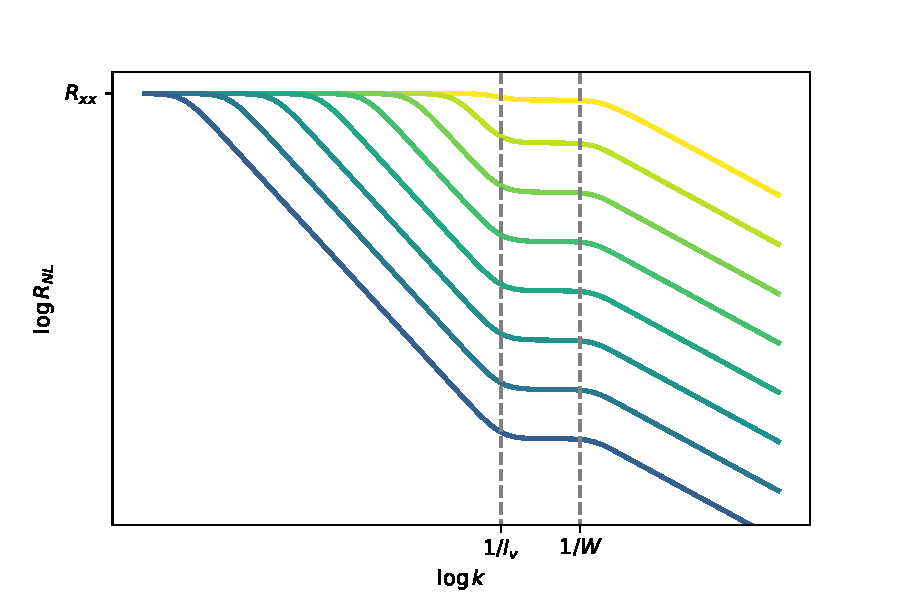
\includegraphics[width=\linewidth]{Immagini/rnl/rho2.pdf}
    \caption{In this graph the darker the line color is, the bigger is the value of $\rho$. Notice how, as we increase $\rho$ the first regime becomes more dominant}
    \label{fig:rho2}
\end{figure}\\

As you can see from figure \ref{fig:rho2} are three regimes here. The first one in for $k<l_{\textrm{v}}^{-1}$, the second one is for $l_{\textrm{v}}^{-1}<k<W^{-1}$ and the third one is for $W^{-1}<k$
\subsubsection*{First regime}
In the first regime ($k< l_{\textrm{v}}^{-1}$) $R_{\textrm{NL}}(k)$ is similar to a Lorentzian function.
\begin{equation}
    \lim_{\rho\to\infty} R_{\textrm{NL}}(k)=2\rho
    \bigg\{
        \frac 2W+ l_{\textrm{v}}k^2\frac{\tan^2(\theta_{\textrm{VH}})}{\tanh[W/2l_{\textrm{v}}]}  
    \bigg\}^{-1}
\end{equation}
We can re-parametrize it As
\begin{equation}
    \lim_{\rho\to\infty} R_{\textrm{NL}}(k)=\frac{R_{xx}}{1+(k/\Gamma)^2}
\end{equation}
Where 
\[
    \Gamma=\frac 1 {\tan(\theta_{\textrm{VH}})}\sqrt{\frac 2{l_{\textrm{v}}W} \tanh\bigg(\frac W{2l_{\textrm{v}}}\bigg)}
\]
Therefore $\rho$ and the standard deviation of the Lorentzian $\Gamma$ are inversely proportional.\\
If we do the anti-Fourier transform of this equation to get the position dependent Non-local resistivity we get 
\[
    \mathcal F^{-1}\bigg[\frac{R_{xx}}{1+(k/\Gamma)^2} \bigg]=\frac 12\rho W\Gamma {e^{-|x|\Gamma}}=
\]
\begin{equation}
    =\frac {\rho W}{\tan(\theta_{\textrm{VH}})}\sqrt{\frac 2{l_{\textrm{v}} W}\tanh\bigg(\frac W{2l_{\textrm{v}}}\bigg)}
    \exp\Bigg[
        \frac{-|x|}{\tan(\theta_{\textrm{VH}})}\sqrt{\frac 2{l_{\textrm{v}} W}\tanh\bigg(\frac W{2l_{\textrm{v}}}\bigg)}
    \Bigg]
\end{equation}
Since $\tan(\theta_{\textrm{VH}})=\rho \sigma_{\textrm{v}}$, for $\rho\to +\infty$ the equation above converges pointwise to the following saturation constant $S$
\begin{equation}
    \lim_{\rho\to\infty}\mathcal F^{-1}\bigg[\frac{R_{xx}}{1+(k/\Gamma)^2} \bigg]=\frac 1{\sigma_{\textrm{v}}}\sqrt{\frac {2W}{l_{\textrm{v}}}\tanh\bigg(\frac W{2l_{\textrm{v}}} \bigg)}\equiv S
\end{equation}

\subsubsection*{Second regime and third regime}
Now that we have calculated how it behaves in the regime where is similar to a Lorenztian, let's calculate the second regime. We have already calculated the value the plateau assumes in equation \ref{eq:plateau} 
\begin{equation}
    R_{\textrm{NL}}(k)\approx \rho W\cos^2(\theta_{\textrm{VH}})
    \label{eq:second_regime}
\end{equation}
While in the third and last regime 
\begin{equation}
    R_{\textrm{NL}}(k)\approx \frac{2\rho}k \cos^2(\theta_{\textrm{VH}})
    \label{eq:third_regime}
\end{equation}
\begin{figure}[h!]
    \centering
    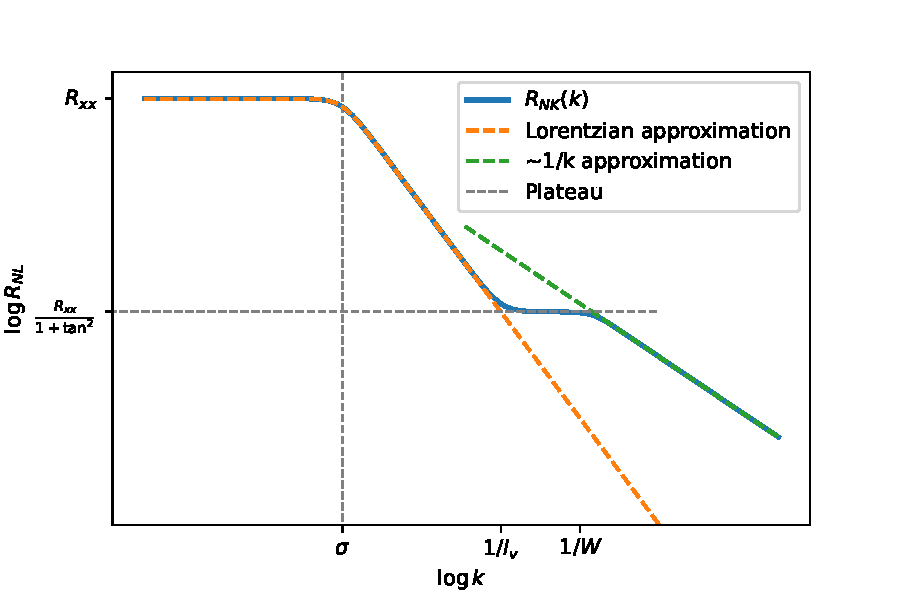
\includegraphics[width=\linewidth]{Immagini/rnl/rho3.pdf}
    \caption{The main regimes of this function}
    \label{fig:rho3}
\end{figure}\\
Notice how the equations for the second and third regime are both proportional to $\rho\cos^2(\theta_{\textrm{VH}})$. This means we can write equation \ref{eq:rhotoinf} as approximately
\begin{equation}
    \lim_{\rho\to\infty} R_{\textrm{NL}}(k)=\frac{R_{xx}}{1+(k/\sigma)^2} + \rho\cos^2(\theta_{\textrm{VH}}) C(k)
    \label{eq:rhotoinf2}
\end{equation}
Where $C(k)$ is a function that doesn't depend on $\rho$ or $\tan(\theta_{\textrm{VH}})$ and it comprehends the second, third regime and eventual corrections in between the approximations\footnote{Yes, the corrections also are proportional to $\rho\cos^2(\theta_{\textrm{VH}})$ SPIEGA PERCHè}.\\
Now let $G(x)$ be it's Fourier anti-transform, then we have that 

\begin{equation}
    \lim_{\rho\to\infty} R_{\textrm{NL}}(x)=S + \frac 1\rho G(x)
\end{equation}
Where here we have used that $\lim_{\rho\to \infty}\rho\cos^2(\theta_{\textrm{VH}})=1/\rho$.
This means that for $\rho\to +\infty$ the right hand side term vanishes, unless it diverges. And indeed $G(x)$ diverges for $x=0$. Therefore, the limit above has pointwise convergence in $\{x\in \mathbb R\,|\,x\neq 0\}$

\begin{equation}
    \lim_{\rho\to\infty} R_{\textrm{NL}}(x) = \frac 1{\sigma_{\textrm{v}}}\sqrt{\frac {2W}{l_{\textrm{v}}}\tanh\bigg(\frac W{2l_{\textrm{v}}} \bigg)}
    \quad\quad \textrm{for }x\neq 0
    \label{eq:highrho}
\end{equation}














\subsection{Putting it all together}
The main result from subsection \ref{sec:lowrho} we showed that for $\tan^2(\theta_{\textrm{VH}})\ll 1$ we had equation \ref{eq:lowrho}
\[
    R_{\textrm{NL}}(x)=
    \frac{2\rho}\pi\ln\bigg |\coth \Big(\frac{\pi x}{2W}\Big)\bigg | +
    \rho^3F(x) +
    o(\rho^5)
\]
While, in subsection \ref{sec:highrho} we had that for $\tan^2(\theta_{\textrm{VH}})\gg \sqrt{1+W^2/(4l_{\textrm{v}}^2)}\tanh\left(\sqrt{1+W^2/(4l_{\textrm{v}}^2)}\right)$ (eq. \ref{eq:highrhocond}) we had equation \ref{eq:highrho}.

\[
    R_{\textrm{NL}}(x) = \frac 1{\sigma_{\textrm{v}}}\sqrt{\frac {2W}{l_{\textrm{v}}}\tanh\bigg(\frac W{2l_{\textrm{v}}} \bigg)}
\]

If we plot the approximations on top of the actual function we get something that looks like figure \ref{fig:all_approx_rho}
\begin{figure}[h!]
    \centering
    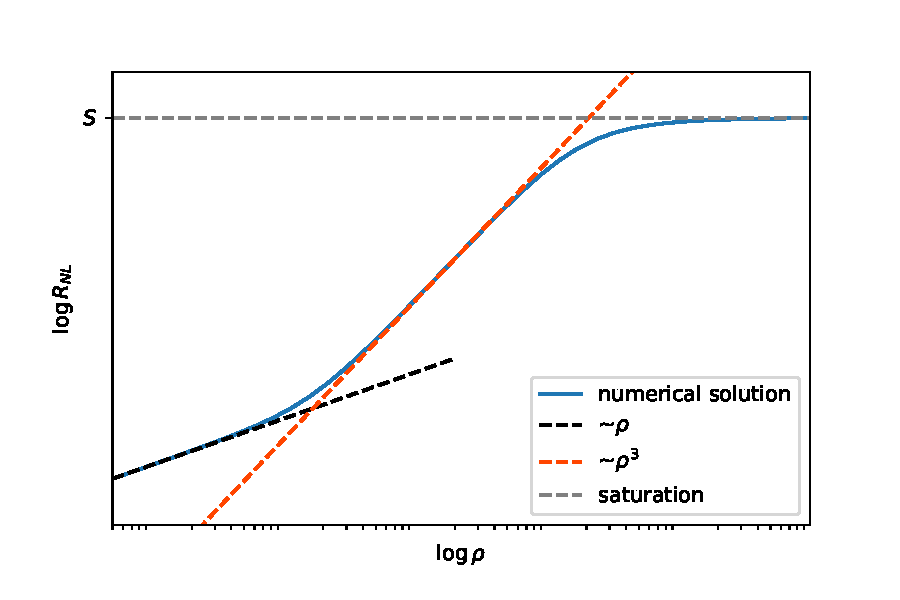
\includegraphics[width=\linewidth]{Immagini/rnl/all_approx_rho.pdf}
    \caption{The main regimes of this function}
    \label{fig:all_approx_rho}
\end{figure}\\

\subsection{Altertative way of studying $R_{\textrm{NL}}(x)$ as we change $\rho$}
Up until now we have studied $R_{\textrm{NL}}(x)$ as we change $\rho$ starting directly from the frequency response function (eq. \ref{eq:rnlk}). This is the most rigorous way for doing this analysis, but it can be cumbersome to work with and doesn't really offer much insight in the topology behind.

A much simpler, but less rigorous way of approaching the problem would be to start from the approximate form of $R_{\textrm{NL}}(x)$ (eq. \ref{eq:rnl}). As you might remeber, this equation had the advantage of being able to distinguish the ohmic effect from the topological ones giving us a strong tool to be able to analyze the graphs.
\begin{figure}[h!]
    \centering
    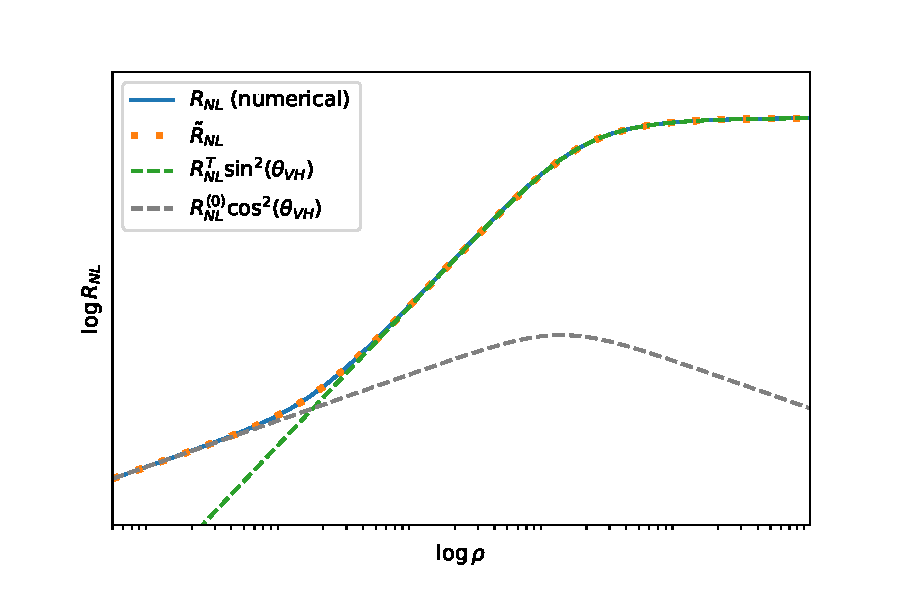
\includegraphics[width=\linewidth]{Immagini/rnl/two_approx_rho.pdf}
    \caption{$R_{\textrm{NL}}$ (continuous blue line, calculated numerically) and its approximation $\tilde R_{\textrm{NL}}$ (dotted orange line) are virtually indistinguishable. The topological component of $\tilde R_{\textrm{NL}}$ is the green dashed line and the ohmic is the grey dashed line.}
    \label{fig:two_approx_rho}
\end{figure}\\

From image \ref{fig:two_approx_rho} it is clear that the linear part at low $\tan(\theta_{\textrm{VH}})$ is due to the ohmic effect. This makes sense even intuitively, infact the current will prefer choosing the path of least resistance, and since at low $\tan(\theta_{\textrm{VH}})$ the ohmic resistivity is much less than the hall resistivity, we have a mostly ohmic behavior.

This image also shows that the topological component is the one responsible for the $\rho^3$ behavior, and then the saturation value.

\subsubsection*{A few small details}
In the discussion about $R_{\textrm{NL}}$ as we change $\rho$ we choose parameters to highlight the behaviors we talked about. However sometimes certain behaviors disappear, for example if we increase the ohmic contributions by decreasing the width of the bar, figures \ref{fig:all_approx_rho} and \ref{fig:two_approx_rho} become like in figure \ref{fig:mixedrho}
\begin{figure}[h!]
    \centering
    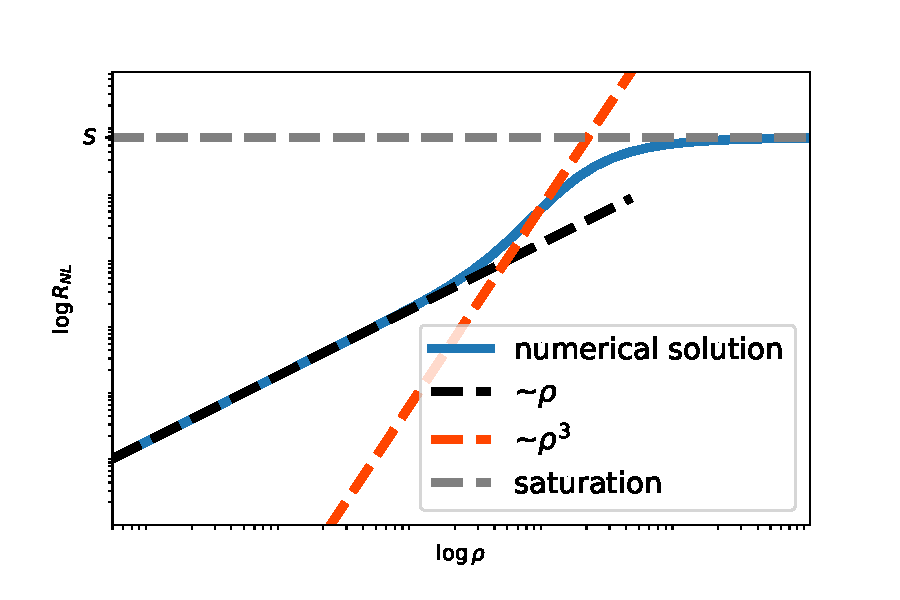
\includegraphics[width=.49\linewidth]{Immagini/rnl/mixed_all_approx_rho.pdf}
    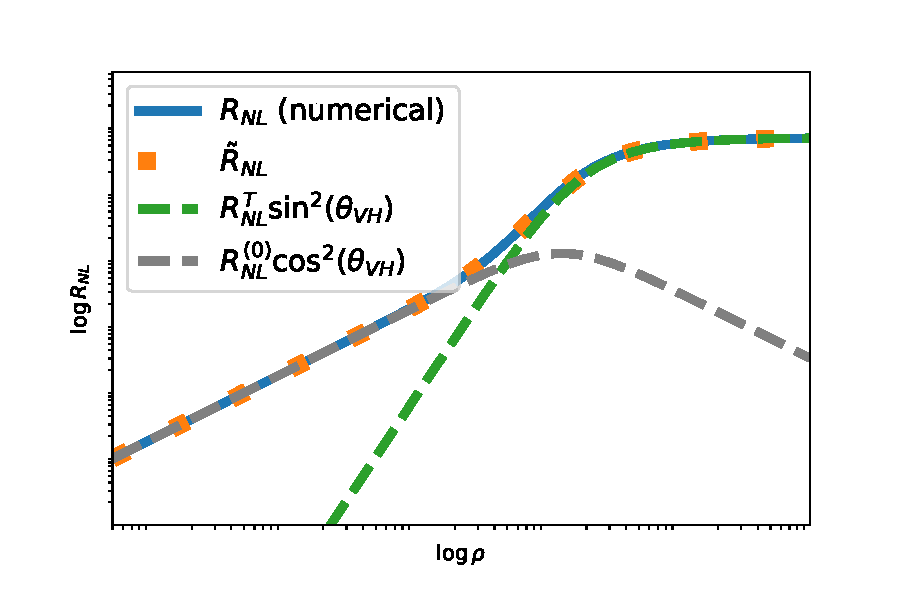
\includegraphics[width=.49\linewidth]{Immagini/rnl/mixed_approx_rho.pdf}
    \caption{As you can see the $\rho^3$ behavior disappeared}
    \label{fig:mixedrho}
\end{figure}\\
In the following section we'll see how this applies to lab measurements
